\section{Teknologi} % (fold)
\label{sec:Teknologi}

I dette afsnit bliver forskellige eksisterende teknologier bearbejdet med henblik på at give et overblik. Hver teknologi vil blive introduceret kort, hvorefter styrker og svagheder vil blive præsenteret. Dette kan senere bruges når en løsning skal designes.


\subsection{Navision} % (fold)
\label{sub:Navision}

Navision eller Microsoft Dynamics NAV er et dansk software regnskabsprogram. Det blev oprindeligt udviklet af Jesper Balser, Torben Wind og Peter Bang tilbage i 1984. Siden da, har det haft forskellige navne. I 2002 opkøbte Microsoft programmet, og integrerede det i deres Microsoft Business Solutions program \cite{visiondata}.

Programmet samler en virksomheds aktiver i en grafisk brugerflade, der gør det enkelt at manipulere data som f.eks.\ medlemmer, materialer og økonomi. Navision er designet til at kunne håndtere alle typer virksomheder, og kan skræddersyes efter behov. Dette sker dog ved besøg af timelønnet programmør.

%\begin{figure}
%  \centering
%  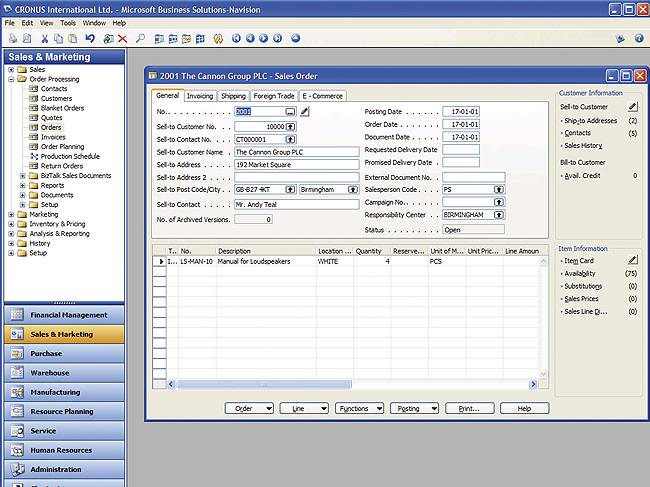
\includegraphics[width=\textwidth]{navision_program.jpg}
%  \caption{Eksempel på Navision program-konfiguration - fra \url{http://www.microsoft.com/business/imagelibrary/businesssolutions/ScreenShotImages/mbs_navision_main_menu_sales.jpg}}alborg kommune har indgået en brugs aftale med Aalborg / Nørresundby Fritidshavn (ANF)
%  \label{fig:navision_program}
%\end{figure}


Et problem med Navision er ifølge Vestre Baadelaug, at man ikke kan lave en regning og sende denne via e-mail \cite{int_vb_sl}. Dette kan dog som tidligere nævnt udbredres ved betaling til supporterende leverandør af Navision.


\subsection{Chip-system} % (fold)
\label{sub:Chip}

I Vestre Baadelaug benyttes et chip-system til at håndtere betalinger fra gæster. Der findes en automat til betaling af pladsbilletter, samt et system til el, bad og toilet.

Billetsystemet giver mulighed for at optanke et kort, eller bestille en dagsbillet. Ved bestilling af dagsbillet, skal systemet vide bådens længde og gæstens nationalitet. Efter endt betaling med kreditkort, udskrives en dagsbillet der skal ligge synligt på båden. Systemet er leveret af det danske firma BEAS. Den specifikke model Vestre Baadelaug benytter er \enquote{Billetautomat TMI}. Se \cref{fig:vb_betalingssystem}.

\begin{figure}
  \centering
  \begin{minipage}{0.45\textwidth}
    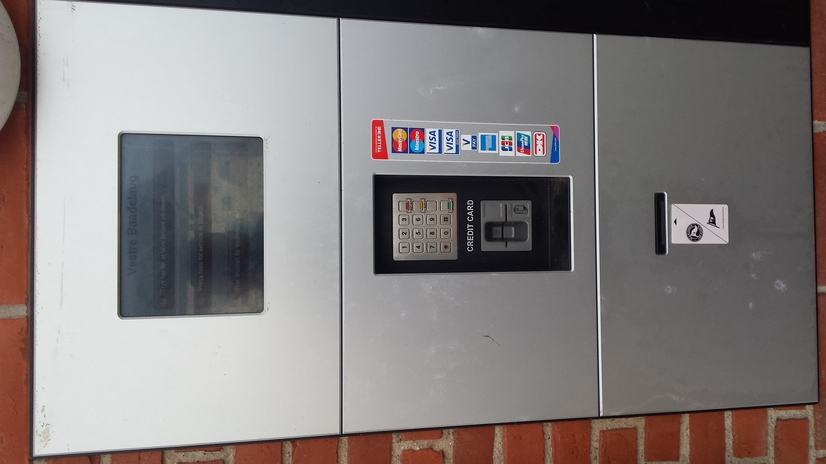
\includegraphics[angle=270,width=\textwidth]{vb_betalingssystem.jpg}
    \caption{Betalingssystem fra BEAS set på Vestre Baadehavn}
    \label{fig:vb_betalingssystem}
  \end{minipage}
  \hfill
  \begin{minipage}{0.45\textwidth}
    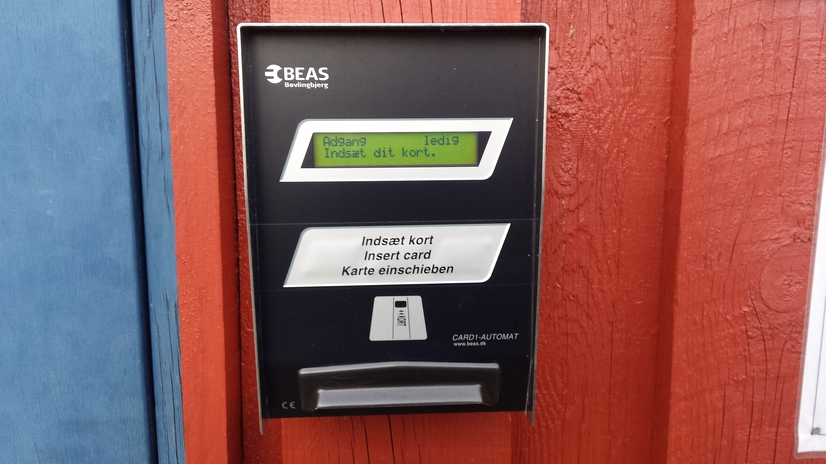
\includegraphics[width=\textwidth]{vb_kortsystem.jpg}
    \caption{Kortsystem fra BEAS set på Vestre Baadehavn}
    \label{fig:vb_kortsystem}
  \end{minipage}
  \begin{minipage}{0.45\textwidth}
    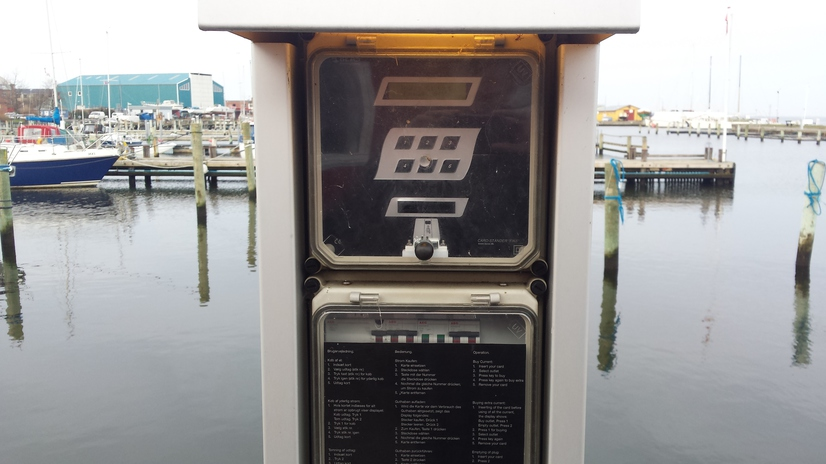
\includegraphics[width=\textwidth]{vb_elsystem.jpg}
    \caption{Elsystem fra BEAS set på Vestre Baadehavn}
    \label{fig:vb_elsystem}
  \end{minipage}
\end{figure}


Derudover benytter Vestre Baadelaug sig også af et chip-system til adgangskontrol til bad- og toiletfaciliteter, samt et system til el. Se \cref{fig:vb_kortsystem,fig:vb_elsystem}.


\subsection{Håndtering af gæster - havnefogeden} % (fold)
\label{sub:havnefogeden}

Når havnefogeden skal holde styr på hvilke gæster der har betalt, benytter han sig af et bånd-system. En mandag kan båndene være f.eks.\ røde, hvorefter de den næste dag kan være blå. På den måde kan havnefogen, når betalende både har synliggjort båndet på deres båd, se om gæsterne har betalt for dagen.

Et andet system havnefogeden bruger, er det der markererer hvorvidt gæster kan fortøje deres båd til en specifik plads. Det virker meget primitivt ved, at når et medlem sejler ud, bliver hans plads ledig, så derfor vender vedkommende et skilt foran pladsen. Dette skilt viser nu grønt, som tegn på at en gæst må holde på pladsen. Det er havnefogedens opgave at få flyttet en eventuel gæst til en anden plads, i tilfælde af at ejeren af pladsen har meddelt havnefogeden, at han kommer hjem tidligere end forventet. Havnefogeden vil så markere pladsen som optaget ved at vende skiltet, så andre gæster ikke tager pladsen.

\subsection{MarinaBooking.dk} % (fold)
\label{sub:MarinaBooking.dk}

Formålet med MarinaBooking \cite{marinabooking} er at gøre vandpladsreservationer lettere for gæster til lystbådehavne i Danmark. Systemet fungerer ved at gæster indtaster ankomst- samt afgangsdato, hvilken havn de vil lægge til og deres båds dimensioner. MarinaBooking kan med disse informationer nu præsentere et oversigtskort over havnebroerne på den specificerede havn, hvor gæsten kan vælge den ønskede vandplads på kortet. Systemet opkræver betaling, og gæsten har nu reserveret denne vandplads.

For at MarinaBooking kan fungere, skal lystbådehavne aktivt tilmelde sig. Dette kan ikke alle havne gøre, f.eks.\ fordi de ikke har en bro udelukkende til gæster  \sinote(link til hvor vi skriver om VB's layout angående gæster/medlemsbro). 

MarinaBooking gør det enkelt for gæster fra Danmark, såvel som fra udlandet, at bestille havepladser fra internettet. Dette er godt for gæsterne, men også for administrationen i havnen, da tildeling af vandpladser herved ordner sig selv.

En af ulemperne ved MarinaBooking er det begrænsede udvalg af samarbejdshavne på hjemmesiden. Dette kan blandt andet skyldes ovenstående forklaring mht.\ gæstebroer.


%\subsection{E-conomic} % (fold)
%\label{sub:e-conomic}

%E-conomic er både navnet på en virksomhed og deres online regnskabsprogram. Formålet med programmet er at gøre økomnomi-håndtering let for selv ikke-regnskabsuddannede. E-conomic henvender sig primært til små- og mellemstore virksomheder \cite{economic}. Prisen for benyttelsen af E-conomic er abonnomentsbaseret med forskellige muligheder for tilpasninger. Da E-conomic kører online i en webbrowser, er alt data gemt og sikkerhedskopieret af E-conomic. Kunden ejer alt data med mulighed for eksportering efter abonnomentsophør.

%Fordelene ved e-conomic er den intuitive brugergrænseflade som letter mange bogførings handlinger. Derudover er programmet skrevet som et web-program hvilket gør at det kan tilgås fra alle platforme samt fra mange lokationer.

%\begin{figure}
%  \centering
%  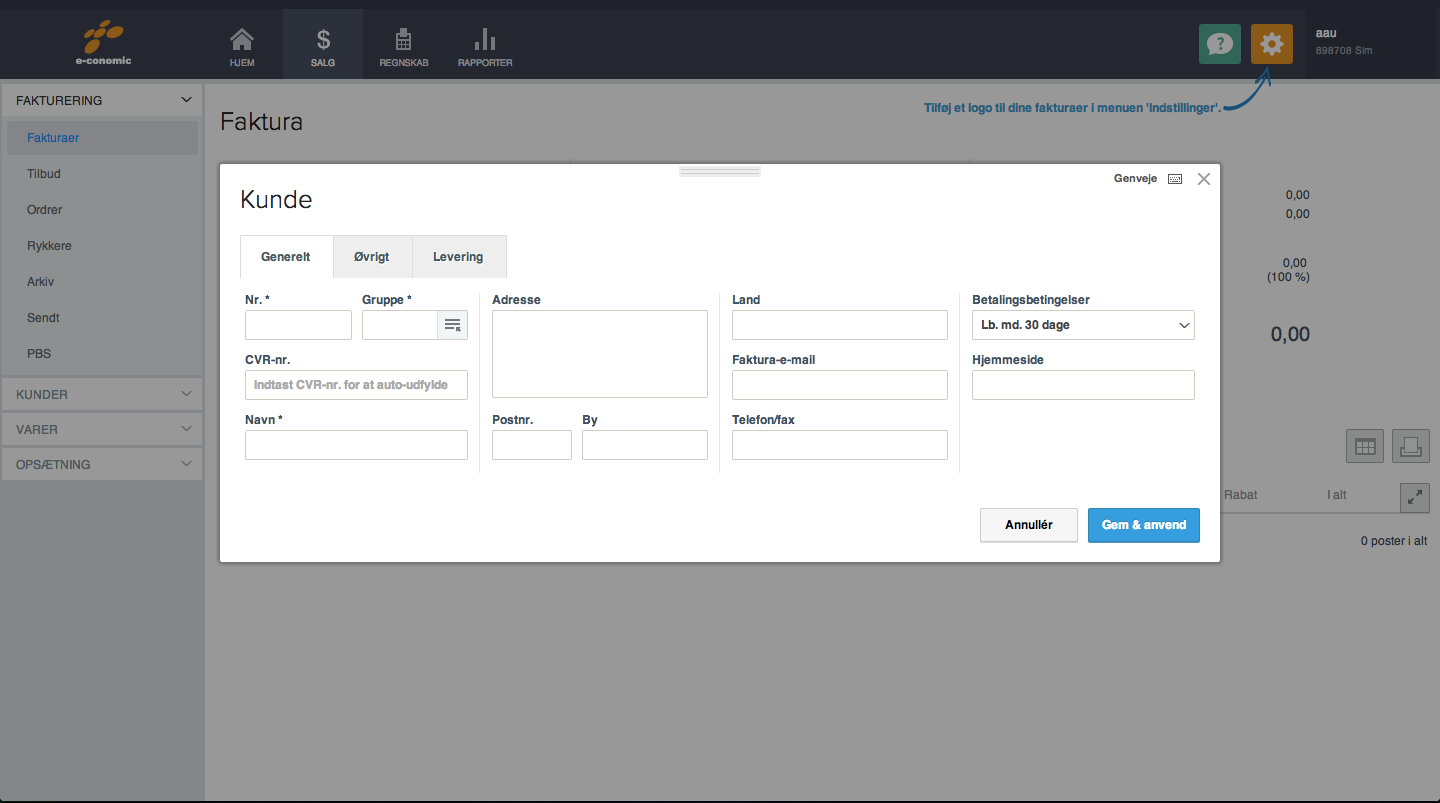
\includegraphics[width=\textwidth]{e-conomic.png}
%  \caption{Brugerinterface ved oprettelse af ny faktura - E-conomic}
%  \label{fig:e_conomic}
%\end{figure}


%Ulemperne ved e-conomic inkluderer afhængigheden af E-conomic med dertilhørende risiko for nedetid. 


\subsection{ForeningLet} % (fold)
\label{sub:ForeningLet}

ForeningLet er et online medlemssystem udviklet af Enteleki. Programmet har, som navnet antyder, specialiseret sig i systemer til foreninger. Det kan blandt andet håndtere medlemmer, regnskab, kontingent opkrævninger og bookning af materialer. Den årlige pris for programmet er afhængigt af antallet af medlemmer i foreningen, og desuden koster tillægsmoduler og dertilhørende ydelser ekstra. F.eks.\ koster et opkrævningsmodul 600 kr./år. Dertil kommer et tillæg på 80 øre per dannet opkrævning. I denne årlige pris er hosting, opdatering og vedligeholdelse inkluderet. ForeningLet holder altså styr på alle medlemsdata og gemmer dette på deres servere \cite{foreninglet}.

Navigationen i programmet foretages i en intuitiv brugerflade i en webbrowser. Man kan altså tilgå programmet på en hvilken som helst enhed med internetforbindelse. 

%\begin{figure}
%  \centering
%  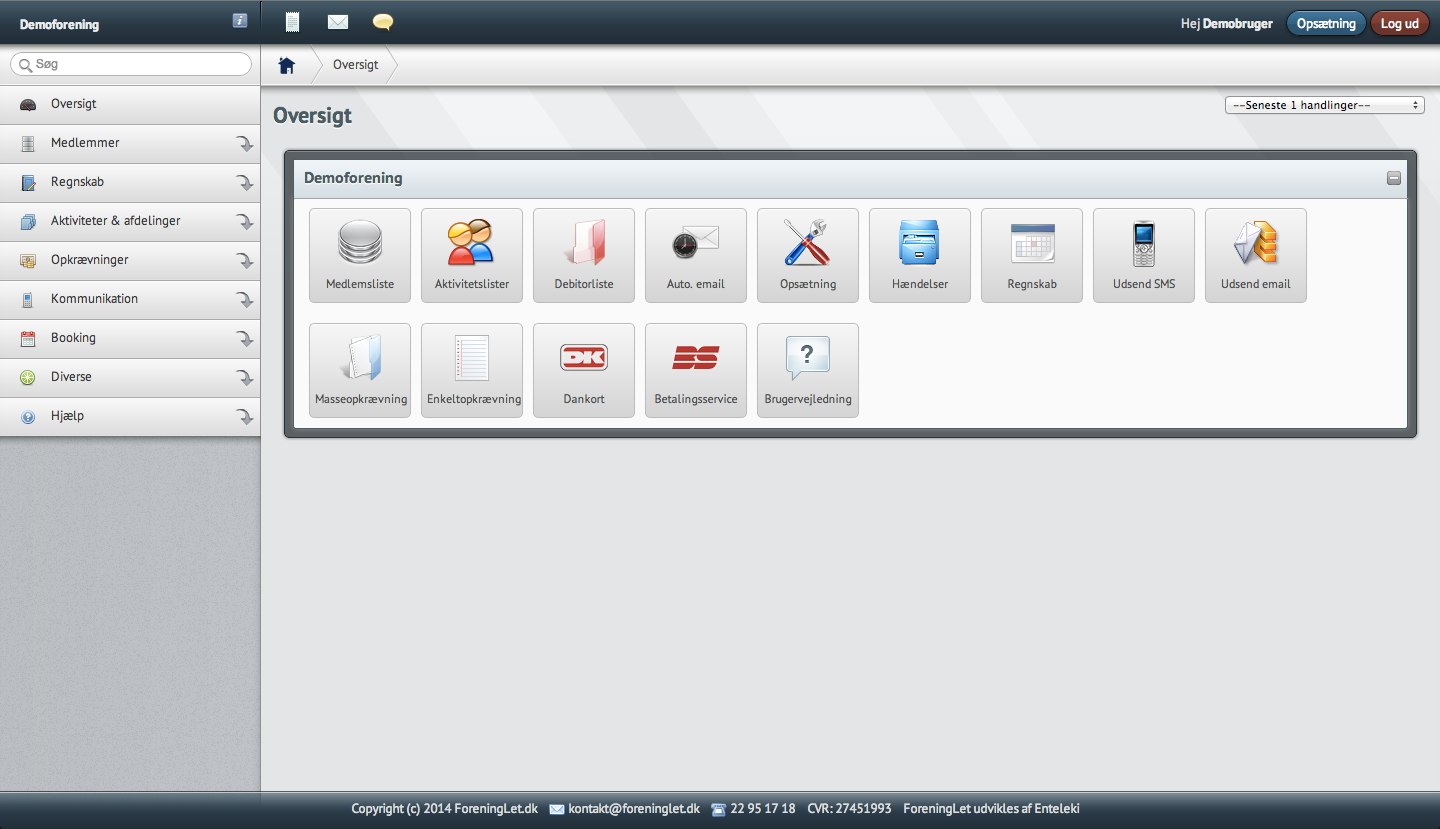
\includegraphics[width=\textwidth]{foreninglet.png}
%  \caption{Oversigt over brugergrænsefladen i ForeningLet}
%  \label{fig:foreninglet_program}
%\end{figure}

Selvom ForeningLet systemet er meget nemt at bruge samt at sætte op, kan det blive dyrt for foreninger med mange medlemmer. Dette skyldes førnævnte gebyrer på tillægsydelser som opkrævninger og rykkere. Derudover er foreningen afgængig af ForeningLet. Dette inkluderer både nedetiden for servicen og at datasikkerhedskopiering fungerer.
% subsection ForeningLet (end)

% section Teknologi (end)
